% GDZ PPN236018647,native519lower–522upper;HKUST520–523.
\NumberedItem{7}
\indent Transformatio seriei
\[
1-2+8-64\ldotp\,\ldotp\,\ldotp
\]
\noindent in fractionem continuam:
\begin{center}
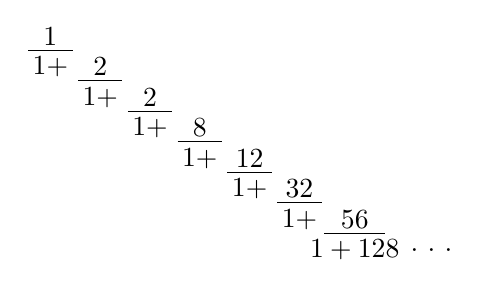
\begin{tikzpicture}[x=1em,y=1em]
\node[inner sep=0] at (0,0) {\(1\)};
\draw (-.8,-.5)--(.8,-.5);
\node[inner sep=0] at (0,-1.1) {\(1+\)};
\node[inner sep=0] at (1.8,-1.1) {\(2\)};
\draw (1,-1.6)--(2.6,-1.6);
\node[inner sep=0] at (1.8,-2.2) {\(1+\)};
\node[inner sep=0] at (3.6,-2.2) {\(2\)};
\draw (2.8,-2.7)--(4.4,-2.7);
\node[inner sep=0] at (3.6,-3.3) {\(1+\)};
\node[inner sep=0] at (5.4,-3.3) {\(8\)};
\draw (4.6,-3.8)--(6.2,-3.8);
\node[inner sep=0] at (5.4,-4.4) {\(1+\)};
\node[inner sep=0] at (7.2,-4.4) {\(12\)};
\draw (6.4,-4.9)--(8,-4.9);
\node[inner sep=0] at (7.2,-5.5) {\(1+\)};
\node[inner sep=0] at (9,-5.5) {\(32\)};
\draw (8.2,-6)--(9.8,-6);
\node[inner sep=0] at (9,-6.6) {\(1+\)};
\node[inner sep=0] at (11,-6.6) {\(56\)};
\draw (9.9,-7.1)--(12.1,-7.1);
\node[inner sep=0] at (11,-7.7) {\(1+128\)};
\node[anchor=west,inner sep=0] at (13,-7.7) {\(\ldotp\,\ldotp\,\ldotp\)};
\end{tikzpicture}
\end{center}

\clearpage\SourceLeaf{520}\ArithmeticHead{491}{R}{1796 MAI. 14—1796 MAI. 24.}
\[
1-1+1.3-1.3.7+1.3.7.15+\ldotp\,\ldotp\,\ldotp
\]
\begin{center}
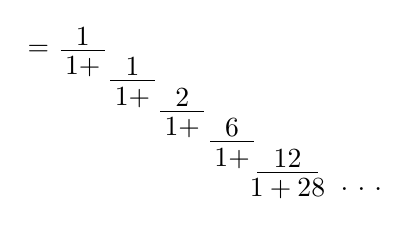
\begin{tikzpicture}[x=1em,y=1em]
\node[inner sep=0] at (-1.6,-.5) {\(=\)};
\node[inner sep=0] at (0,0) {\(1\)};
\draw (-.8,-.5)--(.8,-.5);
\node[inner sep=0] at (0,-1.1) {\(1+\)};
\node[inner sep=0] at (1.8,-1.1) {\(1\)};
\draw (1,-1.6)--(2.6,-1.6);
\node[inner sep=0] at (1.8,-2.2) {\(1+\)};
\node[inner sep=0] at (3.6,-2.2) {\(2\)};
\draw (2.8,-2.7)--(4.4,-2.7);
\node[inner sep=0] at (3.6,-3.3) {\(1+\)};
\node[inner sep=0] at (5.4,-3.3) {\(6\)};
\draw (4.6,-3.8)--(6.2,-3.8);
\node[inner sep=0] at (5.4,-4.4) {\(1+\)};
\node[inner sep=0] at (7.4,-4.4) {\(12\)};
\draw (6.3,-4.9)--(8.5,-4.9);
\node[inner sep=0] at (7.4,-5.5) {\(1+28\)};
\node[anchor=west,inner sep=0] at (9.3,-5.5) {\(\ldotp\,\ldotp\,\ldotp\)};
\end{tikzpicture}
\end{center}
\noindent et aliae.
\par\noindent\hfill[1796] Mai. 24.\quad G[ottingae]

\medskip\begingroup\small\makeatletter\let\veqno\@@leqno\makeatother
\indent In sein Exemplar von \textsc{Lamberts} \textit{Tafeln} hat \textsc{Gauss} die Umformung der divergenten Reihe
\begin{equation*}\tag*{(1)}
1-mx+m.\overline{m+n}xx-m.\overline{m+n}.\overline{m+2n}x^3+\text{ etc. in inf.}
\end{equation*}
\noindent in den Kettenbruch
\begin{center}
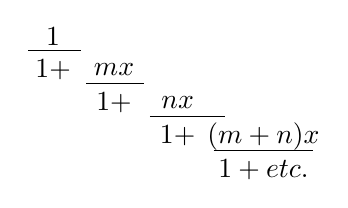
\begin{tikzpicture}[x=1em,y=1em]
\node[inner sep=0] at (0,0) {\(1\)};
\draw (-.9,-.5)--(1,-.5);
\node[inner sep=0] at (0,-1.2) {\(1+\)};
\node[inner sep=0] at (2.2,-1.2) {\(mx\)};
\draw (1.2,-1.7)--(3.3,-1.7);
\node[inner sep=0] at (2.2,-2.4) {\(1+\)};
\node[inner sep=0] at (4.5,-2.4) {\(nx\)};
\draw (3.5,-2.9)--(6.2,-2.9);
\node[inner sep=0] at (4.5,-3.6) {\(1+\)};
\node[inner sep=0] at (7.6,-3.6) {\((m+n)x\)};
\draw (5.8,-4.1)--(9.4,-4.1);
\node[inner sep=0] at (7.6,-4.8) {\(1+\text{etc.}\)};
\end{tikzpicture}
\end{center}
\noindent eingetragen, die \textsc{Euler} zuerst in seiner Abhandlung \textit{De seriebus divergentibus}, Novi Comment. Acad. Petrop. \textbf{5} (1754/55) 1760, S. 205, siehe besonders S. 232, als Verallgemeinerung der analogen Umformung der Reihe
\begin{equation*}\tag*{(1a)}
1-1x+1.2x^2-1.2.3x^3+1.2.3.4x^4-\ldotp\,\ldotp\,\ldotp\text{ in inf.}
\end{equation*}
\noindent behandelt hatte\footnote{\textsc{Euler} ist später auf jene Reihe (1) in einer besondern Abhandlung Nova Acta Acad. Petrop. \textbf{2} (1784) 1788, S. 36 zurückgekommen. Auf die »Summation« der Reihe (1a) für \(x=1\) bezieht sich die oben S. 382 abgedruckte Aufzeichnung von \textsc{Gauss}, vergl. die zugehörige Bemerkung S. 385. Die Umformung der Reihe (1) in den Kettenbruch gibt \textsc{Gauss} auch im art. 14. der \textit{Disquisitiones circa seriem}, 1812, Werke III, S. 138, Gl. [86].}. Den \textsc{Euler}schen Gedanken der Umformung einer divergenten Reihe in einen Kettenbruch wendet \textsc{Gauss} in unsrer Tagebuchaufzeichnung auf zwei Beispiele an. Bei beiden erweist sich aber nicht nur die Reihe, sondern auch der Kettenbruch als divergent. Auf das erste Beispiel kommen wir in der Bemerkung zu der Aufzeichnung Nr. 58 vom 16. Februar 1797 zurück, in Bezug auf das zweite Beispiel ist folgendes zu bemerken.

\indent An der erwähnten Stelle von \textsc{Gauss}' Exemplar der \textsc{Lambert}schen Tafeln findet sich auch die Umformung:
\begin{equation*}\tag*{(2)}
x-axx+abx^3-abcx^4+\text{etc.}
\end{equation*}
\begin{center}
\begin{tikzpicture}[x=1em,y=1em]
\node[inner sep=0] at (-1.8,-.5) {\(=\)};
\node[inner sep=0] at (0,0) {\(1\)};
\draw (-.9,-.5)--(1,-.5);
\node[inner sep=0] at (0,-1.5) {\(\dfrac1x\)};
\node[inner sep=0] at (.9,-1.5) {\(+\)};
\node[inner sep=0] at (2.2,-1.5) {\(1\)};
\draw (1.2,-2)--(3.3,-2);
\node[inner sep=0] at (2.2,-3) {\(\dfrac1a\)};
\node[inner sep=0] at (3.1,-3) {\(+\)};
\node[inner sep=0] at (4.7,-3) {\(1\)};
\draw (3.7,-3.5)--(7.7,-3.5);
\node[inner sep=0] at (5.2,-4.7) {\(\dfrac{a}{b-a}\dfrac1x\)};
\node[inner sep=0] at (7.5,-4.7) {\(+\)};
\node[inner sep=0] at (9.2,-4.7) {\(1\)};
\draw (8.2,-5.2)--(12.8,-5.2);
\node[inner sep=0] at (10,-6.4) {\(\dfrac{(b-a)^2}{ab(c-b)}\)};
\node[inner sep=0] at (12.5,-6.4) {\(+\)};
\node[inner sep=0] at (14.3,-6.4) {\(1\)};
\draw (13.3,-6.9)--(18.5,-6.9);
\node[inner sep=0] at (17,-9.1) {\(\dfrac{ab(c-b)^2\dfrac1x}{(b-a)\{cd(b-a)-bc(c-a)+ab(c-b)\}}\)};
\node[anchor=west,inner sep=0] at (28,-9.1) {\(+\text{etc.}\)};
\end{tikzpicture}
\end{center}
\par\vfill\noindent\hfill62\textsuperscript{*}
\par\endgroup

\clearpage\SourceLeaf{521}\ArithmeticHead{492}{L}{TAGEBUCH MIT ERLÄUTERUNGEN.}
\begingroup\small\makeatletter\let\veqno\@@leqno\makeatother
\noindent Mit Hilfe dieser Formel kann für
\[
a=2^1-1,\quad b=2^2-1,\quad c=2^3-1,\quad\ldotp\,\ldotp\,\ldotp
\]
\noindent das Beispiel unsrer Tagebuchaufzeichnung gerechnet werden. Setzt man allgemein
\begin{equation*}\tag*{(3)}
c_0x-c_1x^2+c_2x^3-c_3x^4+\ldotp\,\ldotp\,\ldotp\text{ in inf.}
\end{equation*}
\begin{center}
\begin{tikzpicture}[x=1em,y=1em,baseline=(current bounding box.north)]
\node[inner sep=0] at (-1.5,-.5) {\(=\)};
\node[inner sep=0] at (0,0) {\(1\)};
\draw (-.8,-.5)--(1,-.5);
\node[inner sep=0] at (0,-1.6) {\(\dfrac{a_1}{x}\)};
\node[inner sep=0] at (1,-1.6) {\(+\)};
\node[inner sep=0] at (2.5,-1.6) {\(1\)};
\draw (1.5,-2.1)--(3.5,-2.1);
\node[inner sep=0] at (2.5,-2.9) {\(a_2+\)};
\node[inner sep=0] at (4.7,-2.9) {\(1\)};
\draw (3.7,-3.4)--(5.8,-3.4);
\node[inner sep=0] at (4.7,-4.5) {\(\dfrac{a_3}{x}\)};
\node[inner sep=0] at (5.8,-4.5) {\(+\)};
\node[inner sep=0] at (7.7,-4.5) {\(1\)};
\draw (6.7,-5)--(10,-5);
\node[inner sep=0] at (8.4,-5.8) {\(a_4+\text{etc.}\)};
\end{tikzpicture}
\qquad
\begin{tikzpicture}[x=1em,y=1em,baseline=(current bounding box.north)]
\node[inner sep=0] at (-1.5,-.5) {\(=\)};
\node[inner sep=0] at (0,0) {\(b_0\)};
\draw (-.8,-.5)--(1,-.5);
\node[inner sep=0] at (0,-1.6) {\(\dfrac1x\)};
\node[inner sep=0] at (1,-1.6) {\(+\)};
\node[inner sep=0] at (2.5,-1.6) {\(b_1\)};
\draw (1.5,-2.1)--(3.6,-2.1);
\node[inner sep=0] at (2.5,-2.9) {\(1+\)};
\node[inner sep=0] at (4.7,-2.9) {\(b_2\)};
\draw (3.7,-3.4)--(5.8,-3.4);
\node[inner sep=0] at (4.7,-4.5) {\(\dfrac1x\)};
\node[inner sep=0] at (5.8,-4.5) {\(+\)};
\node[inner sep=0] at (7.3,-4.5) {\(b_3\)};
\draw (6.3,-5)--(8.5,-5);
\node[inner sep=0] at (7.3,-5.8) {\(1+\)};
\node[inner sep=0] at (9.7,-5.8) {\(b_4\)};
\draw (8.6,-6.3)--(12,-6.3);
\node[inner sep=0] at (10.3,-7.4) {\(\dfrac1x+\text{etc.}\)};
\end{tikzpicture}
\end{center}
\noindent so ist
\begin{equation*}\tag*{(4)}
b_0=c_0=\frac1{a_1},\quad b_1=\frac1{a_1a_2},\quad b_2=\frac1{a_2a_3},\quad\ldotp\,\ldotp\,\ldotp,\quad b_m=\frac1{a_ma_{m+1}},\quad\ldotp\,\ldotp\,\ldotp
\end{equation*}
\noindent und zur Bestimmung der \(a_2,a_3,\ldotp\,\ldotp\,\ldotp\) dienen die bekannten Formeln\footnote{Siehe z. B. T.-J. \textsc{Stieltjes}, \textit{Recherches sur les fractions continues}, Annales de la Faculté des Sciences de Toulouse \textbf{8}, 1894, Abhandlung J., S. 26.}
\begin{equation*}\tag*{(5)}
a_{2n}=\frac{A_n^2}{B_nB_{n-1}},\quad a_{2n+1}=\frac{B_n^2}{A_nA_{n+1}}\qquad(n=1,2,3,\ldotp\,\ldotp\,\ldotp),
\end{equation*}
\noindent wo \(A_0,B_0\) gleich 1 ist und für \(n\geqq1\) die Determinantendarstellungen
\begin{equation*}\tag*{(6)}
A_n=|c_{i+k-2}|,\quad B_n=|c_{i+k-1}|\qquad(i,k=1,2,\ldotp\,\ldotp\,\ldotp,n)
\end{equation*}
\noindent gelten. Für das \textsc{Gauss}sche Beispiel, d. h. für
\begin{equation*}\tag*{(7)}
c_0=1,\quad c_k=1(2-1)(2^2-1)\ldotp\,\ldotp\,\ldotp(2^k-1)\qquad(k=1,2,3,\ldotp\,\ldotp\,\ldotp)
\end{equation*}
\noindent findet man\begingroup\renewcommand{\thefootnote}{**)}\footnote{Die Berechnung der Determinanten \(A_n,B_n\) gestaltet sich am einfachsten, wenn man beachtet, daß für die Determinanten
\[
(\nu,n)=|c_{\nu+i+k-2}|\qquad(i,k=1,2,\ldotp\,\ldotp\,\ldotp,n)
\]
die Rekursionsformel
\[
(\nu,n)=c_\nu.c_{n-1}\,2^{(n-1)\nu+\frac12n(n-1)}(\nu+1,n-1)
\]
gilt, aus der sich sofort
\[
\begin{aligned}
(\nu,n)={}&c_\nu c_{\nu+1}\ldotp\,\ldotp\,\ldotp c_{\nu+n-1}c_{n-1}c_{n-2}\ldotp\,\ldotp\,\ldotp c_1\,.
\\[-2pt]&2^{\frac12n(n-1)(n+\nu-1)-\frac16(n-2)(n-1)n}
\end{aligned}
\]
ergibt. Man hat dann
\[
A_n=(0,n),\quad B_n=(1,n).
\]
}\endgroup\ die Werte
\begin{equation*}\tag*{(8)}
a_{2n}=\frac1{2^n-1},\quad a_{2n+1}=\frac1{2^n}\qquad(n=1,2,3,\ldotp\,\ldotp\,\ldotp),
\end{equation*}
\noindent also in Übereinstimmung mit den Angaben von \textsc{Gauss}:
\[
b_0=1,\quad b_1=1,\quad b_2=2,\quad b_3=6,\quad b_4=12,\quad b_5=28
\]
\noindent und allgemein
\[
b_{2n}=2^{2n}-2^n,\quad b_{2n+1}=2^n(2^{n+1}-1).
\]
\par\endgroup

\clearpage\SourceLeaf{522}\ArithmeticHead{493}{R}{1796 MAI. 24—1796 MAI. 31.}
\begingroup\small\makeatletter\let\veqno\@@leqno\makeatother
\noindent Aus der Konvergenz der mit den Werten (8) gebildeten Reihe \(\displaystyle\sum_{k=1}^{\infty}a_k\) folgt nach M. A. \textsc{Stern}\footnote{Siehe \textsc{Stern}, \textit{Über die Kennzeichen der Convergenz eines Kettenbruchs}, \textsc{Crelles} Journal für Mathem. \textbf{37}, 1848, S. 255, besonders S. 260.} die \textls[120]{Divergenz} des mit eben diesen Werten gebildeten Kettenbruchs für jeden Wert von \(z=\dfrac1x\). Für \(z=1\) ergibt sich das \textsc{Gauss}sche Beispiel. Da die \(a_k\) positiv sind, so ist auf den divergenten Kettenbruch die Theorie von \textsc{Stieltjes}\begingroup\renewcommand{\thefootnote}{**)}\footnote{Siehe a. a. O. S. 36 ff.}\endgroup anwendbar.
\par\noindent\hfill\textsc{Schlesinger}.
\par\endgroup
